\subsection{实验目的}
理解遥感图像目标检测的概念,根据实验七中完成的实验数据,即二值检测结果,完成检测结果的后处理。包括连通分量提取与分析,目标像素聚类,以及目标切片的提取与显示等。
\subsection{实验原理}
\subsubsection{目标检测的一般流程}
\begin{figure}[H]
	\centering
	\begin{tikzpicture}[node distance=4cm]
	\node[process](raw_rs_img){原始遥感图像};
	\node[process, right of=raw_rs_img](binary_img){二值检测结果图像};
	\node[process, right of=binary_img](abstract_obj){候选目标提取};
	\node[process, right of=abstract_obj](remove_false_alert){虚警去除};
	
	\draw[->] (raw_rs_img) -- (binary_img);
	\draw[->] (binary_img) -- (abstract_obj);
	\draw[->] (abstract_obj) -- (remove_false_alert);
	\end{tikzpicture}
\end{figure}
\subsubsection{连通分量的提取}
\begin{figure}[H]
	\centering
	\begin{minipage}{0.45\linewidth}
		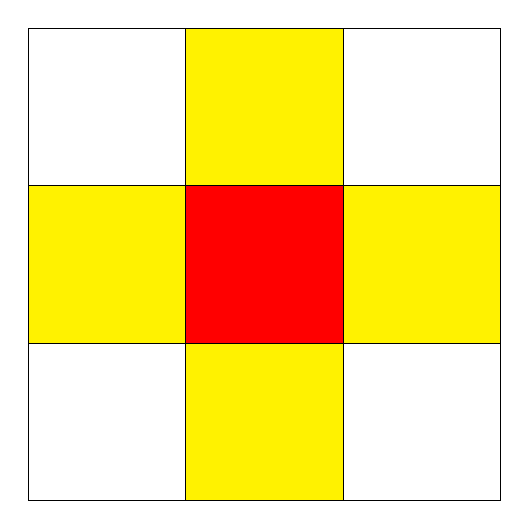
\begin{tikzpicture}
		\draw (0, 0) rectangle ++(6, 6);
		\filldraw[color=yellow, draw=black] (0, 2) rectangle ++(2, 2);
		\filldraw[color=yellow, draw=black] (2, 4) rectangle ++(2, 2);
		\filldraw[color=yellow, draw=black] (4, 2) rectangle ++(2, 2);
		\filldraw[color=yellow, draw=black] (2, 0) rectangle ++(2, 2);
		\filldraw (2, 2)[color=red, draw=black] rectangle ++(2, 2);
		\end{tikzpicture}
		\caption{四邻域}
	\end{minipage}
	\begin{minipage}{0.45\linewidth}
		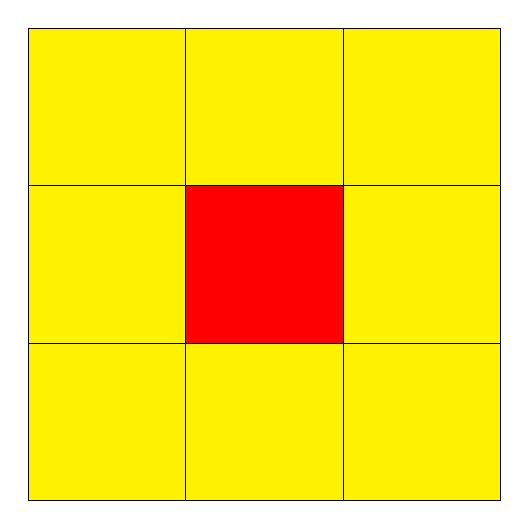
\begin{tikzpicture}
		\draw (0, 0) rectangle ++(6, 6);
		\filldraw (0, 0)[color=yellow, draw=black] rectangle ++(2, 2);
		\filldraw (0, 2)[color=yellow, draw=black] rectangle ++(2, 2);
		\filldraw (0, 4)[color=yellow, draw=black] rectangle ++(2, 2);
		\filldraw (2, 0)[color=yellow, draw=black] rectangle ++(2, 2);
		\filldraw (2, 2)[color=red, draw=black] rectangle ++(2, 2);
		\filldraw (2, 4)[color=yellow, draw=black] rectangle ++(2, 2);
		\filldraw (4, 0)[color=yellow, draw=black] rectangle ++(2, 2);
		\filldraw (4, 2)[color=yellow, draw=black] rectangle ++(2, 2);
		\filldraw (4, 4)[color=yellow, draw=black] rectangle ++(2, 2);
		\end{tikzpicture}
		\caption{八邻域}
	\end{minipage}
\end{figure}
\begin{description}
	\item[连通性] 两个像素是否连通取决于它们是否相邻以及它们的灰度值是否满足特定的相似性准则。
	\item[区域] 图像中的一个像素子集$\mathbb{R}$,该子集是一个连通集,则称$\mathbb{R}$为一个区域。
	\item[连通量] 具有相同输入值的邻接像素的区域。
	\item[连通分量的提取] 对每一个连通量,或每一个连通集$\mathbb{R}$赋予不同的标记。方便对$\mathbb{R}$进行分析。
	\item[$\mathbb{R}$的统计量] 面积,周长,质心,二阶矩等。最小外接矩形,$\mathbb{R}$区域的长度、宽度、长宽比。
\end{description}
\subsubsection{二值检测结果分析}
\begin{enumerate}
	\item 根据目标的大小,形状的先验知识,去除过大或过小的,形状不符合的连通区域。
	\item 对剩余的连通区域进行聚类,得到属于同一个目标的连通区域。
	\item 根据属于同一个目标的连通区域确定目标的中心。
	\item 以目标中心为中心切出目标候选切片。
	\item 进一步分析目标候选切片以去除虚警。
\end{enumerate}
连通区域聚类,得到属于同一个目标的连通区域。
\paragraph{层次聚类法}
\begin{enumerate}
	\item 每个连通区域自成一类,计算两辆距离,得到距离矩阵。
	\item 寻找距离最近的两个连通区域,划为一类。更新类别标记。
	\item 重新计算距离矩阵。
	\item 跳至步骤2,重复计算及合并。结束准则:最小距离大于一个阈值$T$。
\end{enumerate}
\subsection{实验流程}
\subsection{实验程序}
\subsection{实验结果和分析}